% Options for packages loaded elsewhere
% Options for packages loaded elsewhere
\PassOptionsToPackage{unicode}{hyperref}
\PassOptionsToPackage{hyphens}{url}
%
\documentclass[
  11pt,
  ignorenonframetext,
  aspectratio=169,
]{beamer}
\newif\ifbibliography
\usepackage{pgfpages}
\setbeamertemplate{caption}[numbered]
\setbeamertemplate{caption label separator}{: }
\setbeamercolor{caption name}{fg=normal text.fg}
\beamertemplatenavigationsymbolsempty
% remove section numbering
\setbeamertemplate{part page}{
  \centering
  \begin{beamercolorbox}[sep=16pt,center]{part title}
    \usebeamerfont{part title}\insertpart\par
  \end{beamercolorbox}
}
\setbeamertemplate{section page}{
  \centering
  \begin{beamercolorbox}[sep=12pt,center]{section title}
    \usebeamerfont{section title}\insertsection\par
  \end{beamercolorbox}
}
\setbeamertemplate{subsection page}{
  \centering
  \begin{beamercolorbox}[sep=8pt,center]{subsection title}
    \usebeamerfont{subsection title}\insertsubsection\par
  \end{beamercolorbox}
}
% Prevent slide breaks in the middle of a paragraph
\widowpenalties 1 10000
\raggedbottom
\AtBeginPart{
  \frame{\partpage}
}
\AtBeginSection{
  \ifbibliography
  \else
    \frame{\sectionpage}
  \fi
}
\AtBeginSubsection{
  \frame{\subsectionpage}
}
\usepackage{iftex}
\ifPDFTeX
  \usepackage[T1]{fontenc}
  \usepackage[utf8]{inputenc}
  \usepackage{textcomp} % provide euro and other symbols
\else % if luatex or xetex
  \usepackage{unicode-math} % this also loads fontspec
  \defaultfontfeatures{Scale=MatchLowercase}
  \defaultfontfeatures[\rmfamily]{Ligatures=TeX,Scale=1}
\fi
\usepackage{lmodern}

\ifPDFTeX\else
  % xetex/luatex font selection
\fi
% Use upquote if available, for straight quotes in verbatim environments
\IfFileExists{upquote.sty}{\usepackage{upquote}}{}
\IfFileExists{microtype.sty}{% use microtype if available
  \usepackage[]{microtype}
  \UseMicrotypeSet[protrusion]{basicmath} % disable protrusion for tt fonts
}{}
\makeatletter
\@ifundefined{KOMAClassName}{% if non-KOMA class
  \IfFileExists{parskip.sty}{%
    \usepackage{parskip}
  }{% else
    \setlength{\parindent}{0pt}
    \setlength{\parskip}{6pt plus 2pt minus 1pt}}
}{% if KOMA class
  \KOMAoptions{parskip=half}}
\makeatother

\usepackage{color}
\usepackage{fancyvrb}
\newcommand{\VerbBar}{|}
\newcommand{\VERB}{\Verb[commandchars=\\\{\}]}
\DefineVerbatimEnvironment{Highlighting}{Verbatim}{commandchars=\\\{\}}
% Add ',fontsize=\small' for more characters per line
\usepackage{framed}
\definecolor{shadecolor}{RGB}{241,243,245}
\newenvironment{Shaded}{\begin{snugshade}}{\end{snugshade}}
\newcommand{\AlertTok}[1]{\textcolor[rgb]{0.68,0.00,0.00}{#1}}
\newcommand{\AnnotationTok}[1]{\textcolor[rgb]{0.37,0.37,0.37}{#1}}
\newcommand{\AttributeTok}[1]{\textcolor[rgb]{0.40,0.45,0.13}{#1}}
\newcommand{\BaseNTok}[1]{\textcolor[rgb]{0.68,0.00,0.00}{#1}}
\newcommand{\BuiltInTok}[1]{\textcolor[rgb]{0.00,0.23,0.31}{#1}}
\newcommand{\CharTok}[1]{\textcolor[rgb]{0.13,0.47,0.30}{#1}}
\newcommand{\CommentTok}[1]{\textcolor[rgb]{0.37,0.37,0.37}{#1}}
\newcommand{\CommentVarTok}[1]{\textcolor[rgb]{0.37,0.37,0.37}{\textit{#1}}}
\newcommand{\ConstantTok}[1]{\textcolor[rgb]{0.56,0.35,0.01}{#1}}
\newcommand{\ControlFlowTok}[1]{\textcolor[rgb]{0.00,0.23,0.31}{\textbf{#1}}}
\newcommand{\DataTypeTok}[1]{\textcolor[rgb]{0.68,0.00,0.00}{#1}}
\newcommand{\DecValTok}[1]{\textcolor[rgb]{0.68,0.00,0.00}{#1}}
\newcommand{\DocumentationTok}[1]{\textcolor[rgb]{0.37,0.37,0.37}{\textit{#1}}}
\newcommand{\ErrorTok}[1]{\textcolor[rgb]{0.68,0.00,0.00}{#1}}
\newcommand{\ExtensionTok}[1]{\textcolor[rgb]{0.00,0.23,0.31}{#1}}
\newcommand{\FloatTok}[1]{\textcolor[rgb]{0.68,0.00,0.00}{#1}}
\newcommand{\FunctionTok}[1]{\textcolor[rgb]{0.28,0.35,0.67}{#1}}
\newcommand{\ImportTok}[1]{\textcolor[rgb]{0.00,0.46,0.62}{#1}}
\newcommand{\InformationTok}[1]{\textcolor[rgb]{0.37,0.37,0.37}{#1}}
\newcommand{\KeywordTok}[1]{\textcolor[rgb]{0.00,0.23,0.31}{\textbf{#1}}}
\newcommand{\NormalTok}[1]{\textcolor[rgb]{0.00,0.23,0.31}{#1}}
\newcommand{\OperatorTok}[1]{\textcolor[rgb]{0.37,0.37,0.37}{#1}}
\newcommand{\OtherTok}[1]{\textcolor[rgb]{0.00,0.23,0.31}{#1}}
\newcommand{\PreprocessorTok}[1]{\textcolor[rgb]{0.68,0.00,0.00}{#1}}
\newcommand{\RegionMarkerTok}[1]{\textcolor[rgb]{0.00,0.23,0.31}{#1}}
\newcommand{\SpecialCharTok}[1]{\textcolor[rgb]{0.37,0.37,0.37}{#1}}
\newcommand{\SpecialStringTok}[1]{\textcolor[rgb]{0.13,0.47,0.30}{#1}}
\newcommand{\StringTok}[1]{\textcolor[rgb]{0.13,0.47,0.30}{#1}}
\newcommand{\VariableTok}[1]{\textcolor[rgb]{0.07,0.07,0.07}{#1}}
\newcommand{\VerbatimStringTok}[1]{\textcolor[rgb]{0.13,0.47,0.30}{#1}}
\newcommand{\WarningTok}[1]{\textcolor[rgb]{0.37,0.37,0.37}{\textit{#1}}}

\usepackage{longtable,booktabs,array}
\newcounter{none} % for unnumbered tables
\usepackage{calc} % for calculating minipage widths
\usepackage{caption}
% Make caption package work with longtable
\makeatletter
\def\fnum@table{\tablename~\thetable}
\makeatother
\usepackage{graphicx}
\makeatletter
\newsavebox\pandoc@box
\newcommand*\pandocbounded[1]{% scales image to fit in text height/width
  \sbox\pandoc@box{#1}%
  \Gscale@div\@tempa{\textheight}{\dimexpr\ht\pandoc@box+\dp\pandoc@box\relax}%
  \Gscale@div\@tempb{\linewidth}{\wd\pandoc@box}%
  \ifdim\@tempb\p@<\@tempa\p@\let\@tempa\@tempb\fi% select the smaller of both
  \ifdim\@tempa\p@<\p@\scalebox{\@tempa}{\usebox\pandoc@box}%
  \else\usebox{\pandoc@box}%
  \fi%
}
% Set default figure placement to htbp
\def\fps@figure{htbp}
\makeatother





\setlength{\emergencystretch}{3em} % prevent overfull lines

\providecommand{\tightlist}{%
  \setlength{\itemsep}{0pt}\setlength{\parskip}{0pt}}



 


\setbeamertemplate{navigation symbols}{}
\setbeamertemplate{footline}[frame number]
\setbeamertemplate{itemize items}[circle]
\setbeamertemplate{itemize subitem}[triangle]
\setbeamercolor{frametitle}{fg=black}
\setbeamerfont{frametitle}{series=\bfseries}
\usepackage{amsmath}
\newcommand{\indep}{\perp\!\!\!\perp}
\usepackage{booktabs}
\usepackage{array}
\usepackage{adjustbox}
\newcommand{\src}[1]{\par\vspace{-0.2em}{\tiny\color{gray} Source: #1}\par}
\usepackage{fancyvrb}
\fvset{fontsize=\scriptsize}
\makeatletter
\def\verbatim@font{\scriptsize\ttfamily}
\makeatother
\makeatletter
\@ifpackageloaded{caption}{}{\usepackage{caption}}
\AtBeginDocument{%
\ifdefined\contentsname
  \renewcommand*\contentsname{Table of contents}
\else
  \newcommand\contentsname{Table of contents}
\fi
\ifdefined\listfigurename
  \renewcommand*\listfigurename{List of Figures}
\else
  \newcommand\listfigurename{List of Figures}
\fi
\ifdefined\listtablename
  \renewcommand*\listtablename{List of Tables}
\else
  \newcommand\listtablename{List of Tables}
\fi
\ifdefined\figurename
  \renewcommand*\figurename{Figure}
\else
  \newcommand\figurename{Figure}
\fi
\ifdefined\tablename
  \renewcommand*\tablename{Table}
\else
  \newcommand\tablename{Table}
\fi
}
\@ifpackageloaded{float}{}{\usepackage{float}}
\floatstyle{ruled}
\@ifundefined{c@chapter}{\newfloat{codelisting}{h}{lop}}{\newfloat{codelisting}{h}{lop}[chapter]}
\floatname{codelisting}{Listing}
\newcommand*\listoflistings{\listof{codelisting}{List of Listings}}
\makeatother
\makeatletter
\makeatother
\makeatletter
\@ifpackageloaded{caption}{}{\usepackage{caption}}
\@ifpackageloaded{subcaption}{}{\usepackage{subcaption}}
\makeatother

\usepackage{bookmark}
\IfFileExists{xurl.sty}{\usepackage{xurl}}{} % add URL line breaks if available
\urlstyle{same}
\hypersetup{
  pdftitle={Difference-in-Differences: Covariates and Timing},
  pdfauthor={Professor Ji-Woong Chung},
  hidelinks,
  pdfcreator={LaTeX via pandoc}}


\title{\texorpdfstring{Difference-in-Differences: Covariates and
Timing}{Difference-in-Differences: Covariates and Timing}}
\subtitle{\texorpdfstring{BUSS975: Causal Inference in Financial
Research}{BUSS975: Causal Inference in Financial Research}}
\author{Professor Ji-Woong Chung}
\date{}
\institute{Korea University}

\begin{document}
\frame{\titlepage}


\begin{frame}{Where we left off}
\protect\phantomsection\label{where-we-left-off}
\begin{itemize}
\tightlist
\item
  Lecture 7a: difference-in-differences is \textbf{four averages and
  three subtractions}.
\item
  It identifies the ATT if the two groups' untreated outcomes would have
  moved in parallel, and the baseline is untreated.
\item
  Three regressions gave the same number: the interaction, two-way fixed
  effects (TWFE), the long difference. ``DiD'' and ``TWFE'' were
  synonyms.
\end{itemize}

\vspace{0.5em}

\begin{itemize}
\tightlist
\item
  That equivalence holds for \textbf{one} treated group, \textbf{one}
  control group and \textbf{one} date.
\item
  This lecture and the next ask what happens when the design stops being
  a single \(2 \times 2\).
\item
  Source: Cunningham (2025), \emph{The Remix}, ch.~10; see also Baker et
  al.~(2025).
\end{itemize}
\end{frame}

\begin{frame}{Four ways the single \(2 \times 2\) breaks}
\protect\phantomsection\label{four-ways-the-single-2-times-2-breaks}
\begin{enumerate}
\tightlist
\item
  \textbf{The sample changes under your feet.} Units drop out; a
  repeated cross-section draws different people.
\item
  \textbf{The trends are not parallel}, but a second comparison inside
  the same states might share the bias. \emph{Triple differences.}
\item
  \textbf{The groups differ in ways you can measure.} Parallel trends
  holds only among similar units. \emph{Covariates.}
\item
  \textbf{Treatment arrives at different dates.} TWFE quietly becomes a
  weighted average of comparisons nobody chose.
\end{enumerate}

\vspace{0.5em}

\begin{itemize}
\tightlist
\item
  Today: all four, ending with what TWFE computes under staggered
  timing.
\item
  Lecture 7c: estimators built to avoid its bad comparisons, and how to
  read their event studies.
\end{itemize}
\end{frame}

\section{1. Who Is in the Sample}\label{who-is-in-the-sample}

\begin{frame}{Imbalanced panels: is missing data a problem?}
\protect\phantomsection\label{imbalanced-panels-is-missing-data-a-problem}
\begin{itemize}
\tightlist
\item
  A panel follows the same units. When some drop out or reappear, the
  panel is \textbf{imbalanced}.
\item
  Parallel trends is a statement about the \textbf{average change} in
  \(Y^0\). Missing units matter only if they change that average.
\item
  If units go missing \textbf{at random}, the average is unaffected
  (Wooldridge 2010).
\item
  Weaker and enough: missingness \(M\) is unrelated to the
  \emph{untreated} outcome, given covariates, \[
  Y^0 \;\indep\; M \mid X \qquad\Longrightarrow\qquad \mathbb{E}[Y^0 \mid M=1, X] = \mathbb{E}[Y^0 \mid M=0, X].
  \]
\end{itemize}
\end{frame}

\begin{frame}{Two people who leave}
\protect\phantomsection\label{two-people-who-leave}
\begin{itemize}
\tightlist
\item
  \textbf{Maria} (treated) leaves because the training got her promoted.

  \begin{itemize}
  \tightlist
  \item
    She is missing because of her \(Y^1\), not her \(Y^0\).
  \item
    The untreated trend is untouched. Her absence changes \emph{which}
    treated outcomes we see, not the counterfactual.
  \end{itemize}
\item
  \textbf{Inez} (control) drops out in year 4, for reasons unrelated to
  \(Y^0\) given \(X\).

  \begin{itemize}
  \tightlist
  \item
    Impute her missing \emph{observed} outcome from untreated units like
    her.
  \item
    A missing-data problem, not an identification problem.
  \end{itemize}
\end{itemize}

\vspace{0.4em}

\begin{itemize}
\tightlist
\item
  The rule: know \textbf{why} units are missing before you drop them.
\item
  Chained DiD (Bellego, Benatia and Dortet-Bernadet 2024) links
  adjacent-period changes, under its own assumptions.
\end{itemize}
\end{frame}

\begin{frame}{Repeated cross-sections: did Napster kill music sales?}
\protect\phantomsection\label{repeated-cross-sections-did-napster-kill-music-sales}
\begin{center}
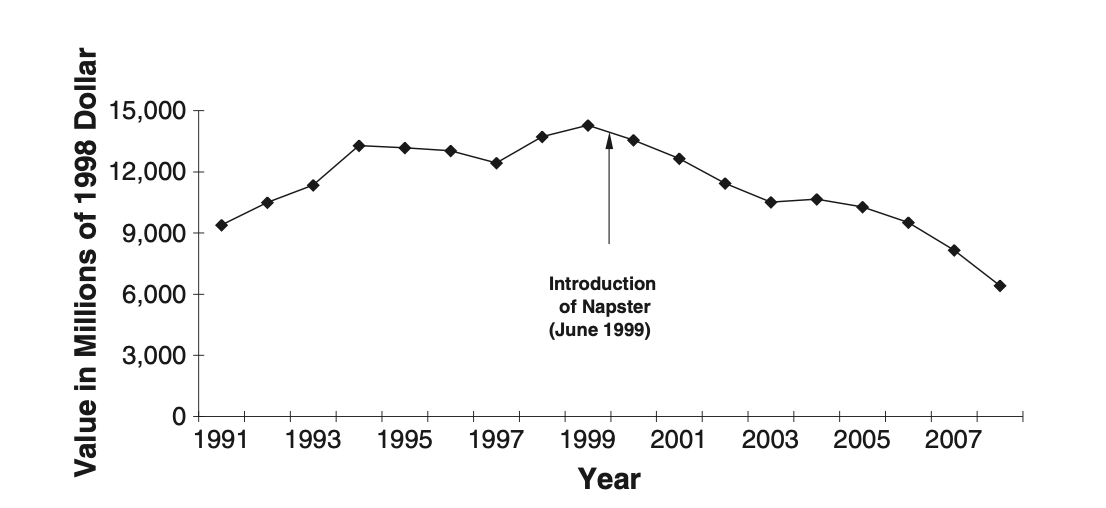
\includegraphics[height=4.3cm]{figs/remix10-01.png}
\end{center}
\src{Hong (2013), reproduced in Cunningham (2025), Figure 10.1.}

\begin{itemize}
\tightlist
\item
  Record sales peak in 1999, the year Napster arrived. Coincidence, or
  cause?
\item
  No geographic variation in access, so Hong compares \textbf{internet
  users} with \textbf{non-users} in the Consumer Expenditure Survey: a
  fresh random sample every year.
\end{itemize}
\end{frame}

\begin{frame}{Who is ``treated'' changes over time}
\protect\phantomsection\label{who-is-treated-changes-over-time}
\begin{center}\small
\begin{tabular}{lcccccccc}
\toprule
 & \multicolumn{2}{c}{1997} & \multicolumn{2}{c}{1998} & \multicolumn{2}{c}{1999} & \multicolumn{2}{c}{2000} \\
 & User & Non & User & Non & User & Non & User & Non \\
\midrule
Age & 40.2 & 49.0 & 42.3 & 49.0 & 44.1 & 49.4 & 44.3 & 49.9 \\
Income (\$000) & 52.9 & 30.5 & 52.0 & 26.2 & 50.0 & 26.6 & 47.5 & 26.3 \\
College graduate & 0.43 & 0.21 & 0.45 & 0.21 & 0.42 & 0.20 & 0.37 & 0.20 \\
\bottomrule
\end{tabular}
\end{center}

\begin{itemize}
\tightlist
\item
  As internet use spread, the ``treated'' group got \textbf{older,
  poorer and less educated}.
\item
  Older people buy less music. So users' spending falls even if Napster
  does nothing.
\item
  Nobody dropped out and nobody anticipated. Parallel trends breaks
  \textbf{because different people are sampled.}
\end{itemize}
\end{frame}

\begin{frame}{Why composition breaks parallel trends}
\protect\phantomsection\label{why-composition-breaks-parallel-trends}
Suppose spending depends on age, \(Y^0 = a + bX + \text{trend}_t\). For
the treated group, \[
\bar Y_{T,\text{post}} - \bar Y_{T,\text{pre}} = \underbrace{\text{trend}}_{\text{same people, new year}} + \underbrace{b\,(\bar X_{T,\text{post}} - \bar X_{T,\text{pre}})}_{\text{different people}} .
\]

\begin{itemize}
\tightlist
\item
  The control group has its own composition term. DiD removes the trend,
  but not the \textbf{difference in composition terms}.
\item
  In a panel the second term is zero by construction: the same people
  are followed.
\item
  In a repeated cross-section it is zero only if each group's mix of
  \(X\) is stable over time.
\end{itemize}
\end{frame}

\begin{frame}{Diagnosing compositional change}
\protect\phantomsection\label{diagnosing-compositional-change}
\begin{itemize}
\tightlist
\item
  \textbf{Diagnostic 1.} A balance table \emph{over time}, like the
  previous one, not just at baseline.
\item
  \textbf{Diagnostic 2.} Run the DiD with an exogenous covariate as the
  \emph{outcome}: \[
  X_{it} = \alpha + \beta_1 D_i + \beta_2 \text{Post}_t + \delta\,(D_i \times \text{Post}_t) + \varepsilon_{it}.
  \]
\item
  Napster cannot make anyone older. A significant \(\hat\delta\) says
  the sample's composition shifted at treatment.
\item
  If that \(X\) also predicts \(Y^0\), parallel trends is mechanically
  broken.
\end{itemize}
\end{frame}

\begin{frame}{Repairing it: reweight each period (Hong 2013)}
\protect\phantomsection\label{repairing-it-reweight-each-period-hong-2013}
\begin{enumerate}
\tightlist
\item
  Estimate \textbf{two} propensity scores, one per period:
  \(P_b = \Pr(D=1 \mid T=0, X)\) and \(P_a = \Pr(D=1 \mid T=1, X)\).
\item
  Compute the four cell means with inverse-probability weights from
  \textbf{their own period's} score.
\item
  Take the \(2 \times 2\) of the weighted means. Equivalently, the usual
  DiD regression by weighted least squares.
\end{enumerate}

\vspace{0.4em}

\begin{itemize}
\tightlist
\item
  Intuition: reweight every year's sample to have the \textbf{same mix
  of \(X\)}. Then the composition term on the previous slide is zero.
\item
  Panels are expensive; much of the world's data are repeated
  cross-sections. This fix deserves more use (see also Sant'Anna and Xu
  2023).
\end{itemize}
\end{frame}

\section{2. Triple Differences}\label{triple-differences}

\begin{frame}{Gruber (1994): who pays for maternity benefits?}
\protect\phantomsection\label{gruber-1994-who-pays-for-maternity-benefits}
\begin{itemize}
\tightlist
\item
  Some states mandated that employer health insurance cover maternity.
\item
  If wages cannot adjust worker by worker, the mandate makes
  childbearing-age women more expensive to hire. Do their wages fall?
\item
  The obvious DiD: married women aged 20--40, mandate states vs.~other
  states, before vs.~after. Writing \(NJ\) for mandate states and \(PA\)
  for the rest, \[
  \hat\delta = \underbrace{D}_{\text{effect}} + \underbrace{(NJ_t - PA_t)}_{\text{non-parallel trends bias}} .
  \]
\item
  Gruber worried that state labour markets were on different paths for
  reasons unrelated to the mandate. Then this DiD is biased.
\end{itemize}
\end{frame}

\begin{frame}{The fix: a second DiD in the same states}
\protect\phantomsection\label{the-fix-a-second-did-in-the-same-states}
\begin{itemize}
\tightlist
\item
  Find a group in the \textbf{same states} that the law does not touch:
  single men aged 20--40 and workers over 40.
\item
  Their DiD has no effect in it, only the bias:
  \(\hat\delta_{\text{alt}} = (NJ_t - PA_t)\).
\item
  Subtract: \[
  \hat\delta_{DDD} = \hat\delta_{\text{primary}} - \hat\delta_{\text{alt}} = D + (NJ_t - PA_t) - (NJ_t - PA_t) = D.
  \]
\item
  Intuition: the second DiD \textbf{measures the bias} of the first.
  Whatever made mandate states' labour markets drift, it shows up for
  the untouched workers too.
\end{itemize}
\end{frame}

\begin{frame}{Two biased DiDs, one unbiased triple difference}
\protect\phantomsection\label{two-biased-dids-one-unbiased-triple-difference}
\begin{center}
\includegraphics[width=0.84\linewidth,height=\textheight,keepaspectratio]{07b_did_covariates_timing_files/figure-beamer/ddd-sim-1.pdf}
\end{center}

\src{Simulated, after Cunningham (2025), Figure 10.3: both groups share a bias of $-500$ a year; true effect $-5{,}000$.}

\begin{itemize}
\tightlist
\item
  Both DiDs show the same falling pre-trend. Their difference (green) is
  flat before and \(-5{,}000\) after.
\end{itemize}
\end{frame}

\begin{frame}{The assumption: parallel bias}
\protect\phantomsection\label{the-assumption-parallel-bias}
\begin{itemize}
\tightlist
\item
  With \(D\) the state and \(G\) the eligible group, DDD needs the
  \textbf{same bias} for both groups (Olden and Møen 2022): \[
  \begin{aligned}
  &\mathbb{E}[\Delta Y^0 \mid D=1, G=1] - \mathbb{E}[\Delta Y^0 \mid D=0, G=1] \\
  &\qquad = \mathbb{E}[\Delta Y^0 \mid D=1, G=0] - \mathbb{E}[\Delta Y^0 \mid D=0, G=0].
  \end{aligned}
  \]
\item
  The second DiD is \textbf{not required to be zero}, only equal to the
  first DiD's bias.
\item
  If it \emph{were} zero, the first DiD was fine all along. The second
  group would then be a falsification (``same outcome, different
  group''), as with Miller, Johnson and Wherry's elderly in 7a.
\item
  So triple differences is a \textbf{design}, not a falsification.
\end{itemize}
\end{frame}

\begin{frame}{Triple differences by regression}
\protect\phantomsection\label{triple-differences-by-regression}
Eight averages and seven subtractions. Identical to OLS with
\textbf{all} interactions of period \(\tau_t\), group \(\delta_g\) and
state \(D_i\): \[
\begin{aligned}
Y_{igt} = \alpha &+ \beta_1\tau_t + \beta_2 \delta_g + \beta_3 D_i + \beta_4(\delta\tau)_{gt} \\
&+ \beta_5(\tau D)_{ti} + \beta_6(\delta D)_{ig} + \beta_7(\delta \tau D)_{igt} + \varepsilon_{igt}.
\end{aligned}
\]

\begin{itemize}
\tightlist
\item
  \(\beta_7\) is the triple difference. Drop any of the two-way terms
  and it no longer is.
\item
  Event study: interact the two- and three-way terms with every period
  except \(\tau = -1\).
\end{itemize}
\end{frame}

\begin{frame}{Triple differences in practice}
\protect\phantomsection\label{triple-differences-in-practice}
\begin{itemize}
\tightlist
\item
  \textbf{Cluster} where the law varies: the state.
\item
  \textbf{Show three event studies}: each DiD, and their difference.
\item
  The two DiDs' pre-trends should look alike. That is the visible part
  of ``parallel bias''.
\item
  Almost nobody shows them. Show yours.
\end{itemize}
\end{frame}

\begin{frame}{Gruber's result}
\protect\phantomsection\label{grubers-result}
\begin{center}\scriptsize
\begin{tabular}{lccc}
\toprule
Log hourly wage & Before & After & Difference \\
\midrule
\multicolumn{4}{l}{\emph{A. Married women 20--40}} \\
Experimental states & 1.547 & 1.513 & $-0.034$ \\
Non-experimental states & 1.369 & 1.397 & $0.028$ \\
Difference-in-differences & & & $\mathbf{-0.062}$ (0.022) \\
\midrule
\multicolumn{4}{l}{\emph{B. Over 40 and single men 20--40}} \\
Experimental states & 1.759 & 1.748 & $-0.011$ \\
Non-experimental states & 1.630 & 1.627 & $-0.003$ \\
Difference-in-differences & & & $\mathbf{-0.008}$ (0.014) \\
\midrule
Triple difference & & & $\mathbf{-0.054}$ (0.026) \\
\bottomrule
\end{tabular}
\end{center}

\begin{itemize}
\tightlist
\item
  Panel B \emph{estimates the bias} of panel A. Here it is small, so DDD
  and DiD nearly agree.
\item
  Married women's wages fell about \(5\) percent: the mandate was paid
  for by the workers it protected.
\item
  No event study in 1994; the practice did not arrive until the 2000s.
\end{itemize}
\end{frame}

\section{3. Covariates}\label{covariates}

\begin{frame}{Levels, trends, and why covariates enter}
\protect\phantomsection\label{levels-trends-and-why-covariates-enter}
\begin{itemize}
\tightlist
\item
  Parallel trends is about trends, not levels. Groups at different
  levels are fine \textbf{in principle}.
\item
  In practice a large level gap is a warning: whatever made the groups
  different might also make their untreated \emph{trends} different.
\item
  Kahn-Lang and Lang (2020): every DiD paper should say why the levels
  differ and why that would not affect the trends.
\item
  Often the \textbf{distribution of covariates} drives both. Then
  condition on them, \textbf{conditional parallel trends} (Heckman,
  Ichimura and Todd 1997): \[
  \mathbb{E}[Y^0_{\text{post}} - Y^0_{\text{pre}} \mid D=1, X] \;=\; \mathbb{E}[Y^0_{\text{post}} - Y^0_{\text{pre}} \mid D=0, X].
  \]
\end{itemize}
\end{frame}

\begin{frame}{What conditioning buys, and what it costs}
\protect\phantomsection\label{what-conditioning-buys-and-what-it-costs}
\begin{itemize}
\tightlist
\item
  \textbf{Buys}: parallel trends only among units with the \textbf{same
  \(X\)}. Young treated workers are compared with young controls, old
  with old.
\item
  \textbf{Costs} two things:

  \begin{itemize}
  \tightlist
  \item
    \textbf{common support}: for every treated \(X\) there must be
    controls with that \(X\), or a functional form that extrapolates
    where there are none;
  \item
    a decision about \textbf{which} \(X\).
  \end{itemize}
\end{itemize}

\vspace{0.4em}

\begin{itemize}
\tightlist
\item
  Example: if young workers' earnings grow faster and the treated are
  mostly young, the raw DiD mixes the treatment effect with an
  age-driven trend. Conditioning on age removes the age-driven part.
\end{itemize}
\end{frame}

\begin{frame}{Which covariates?}
\protect\phantomsection\label{which-covariates}
\begin{center}
\includegraphics[width=0.4\linewidth,height=\textheight,keepaspectratio]{07b_did_covariates_timing_files/figure-beamer/dag-x-1.pdf}
\end{center}

\src{After Cunningham (2025), Figure 10.4.}

\(X\) must do \textbf{both} things:

\begin{enumerate}
\tightlist
\item
  \(X \rightarrow D\): it is distributed differently in treated and
  control groups;
\item
  \(X \rightarrow \Delta \mathbb{E}[Y^0]\): it drives the untreated
  \textbf{trend}.
\end{enumerate}

\begin{itemize}
\tightlist
\item
  Only the first: harmless but useless. Only the second: precision, not
  identification. Both: a confounder of trends.
\end{itemize}
\end{frame}

\begin{frame}{Where the list comes from}
\protect\phantomsection\label{where-the-list-comes-from}
\begin{itemize}
\tightlist
\item
  \textbf{The field} that studies ordinary trends in your outcome.
\item
  \textbf{A DAG} that forces you to say what moves \(Y^0\).
\item
  \textbf{Data-driven selection} fitted \textbf{on untreated units
  only}; Borgschulte and Vogler (2020) use LASSO this way.
\end{itemize}

\vspace{0.4em}

\begin{itemize}
\tightlist
\item
  \textbf{Never} a post-treatment covariate: it may respond to
  treatment. Measure \(X\) at baseline.
\item
  The list can swing the estimate a lot. Fix it before you see results,
  and say so.
\end{itemize}
\end{frame}

\begin{frame}{Is there imbalance? The normalized difference}
\protect\phantomsection\label{is-there-imbalance-the-normalized-difference}
\[
\text{Norm.\ Diff}_\omega = \frac{\bar X_{\omega,T} - \bar X_{\omega,C}}{\sqrt{(S^2_{\omega,T} + S^2_{\omega,C})/2}}
\]

\begin{itemize}
\tightlist
\item
  A difference in means in standard-deviation units, so it does not grow
  with the sample the way a \(t\)-statistic does.
\item
  Rule of thumb: worry when \(|{\cdot}| > 0.25\) (Imbens and Rubin
  2015).
\end{itemize}
\end{frame}

\begin{frame}{Imbalance in the LaLonde data}
\protect\phantomsection\label{imbalance-in-the-lalonde-data}
Lecture 3's job-training data, treated vs.~CPS controls:

\begin{center}\small
\begin{tabular}{lccc}
\toprule
 & Mean treated & Mean control & Norm.\ diff. \\
\midrule
Age & 25.8 & 33.2 & $-0.80$ \\
Education & 10.3 & 12.0 & $-0.68$ \\
Black & 0.84 & 0.07 & $2.43$ \\
Hispanic & 0.06 & 0.07 & $-0.05$ \\
Married & 0.19 & 0.71 & $-1.23$ \\
Unemployed 1974 & 0.71 & 0.12 & $1.49$ \\
\bottomrule
\end{tabular}
\end{center}

\begin{itemize}
\tightlist
\item
  Everything but Hispanic is far past the line.
\item
  Irrelevant if these variables do not drive earnings \emph{trends};
  fatal if they do. Either way, use conditional parallel trends and an
  estimator built for it.
\end{itemize}
\end{frame}

\begin{frame}{Four ways to use conditional parallel trends}
\protect\phantomsection\label{four-ways-to-use-conditional-parallel-trends}
\begin{center}\small
\begin{tabular}{lll}
\toprule
Estimator & What it does & What must be right \\
\midrule
IPW (Abadie 2005) & reweights controls to look like the treated & the propensity score \\
Outcome regression & predicts the treated's $\Delta Y^0$ from controls & the outcome model \\
Doubly robust & both at once & either one of the two \\
TWFE $+\,\theta X$ & adds $X$ linearly to the regression & linearity, constant $\theta$, \\
 & & homogeneous effects \\
\bottomrule
\end{tabular}
\end{center}

\begin{itemize}
\tightlist
\item
  All four target the same thing: the \textbf{counterfactual change} of
  the treated, built from controls with the same \(X\).
\item
  They differ in which side they adjust and what model they trust.
\end{itemize}
\end{frame}

\begin{frame}{Estimator 1: inverse probability weighting (Abadie 2005)}
\protect\phantomsection\label{estimator-1-inverse-probability-weighting-abadie-2005}
Estimate \(p(X) = \Pr(D=1 \mid X_b)\) from \textbf{baseline} covariates.
Then \[
\hat\delta_{IPW} = \mathbb{E}\!\left[\frac{Y_{\text{post}} - Y_{\text{pre}}}{\Pr(D=1)} \cdot \frac{D - p(X)}{1 - p(X)}\right].
\]

\begin{itemize}
\tightlist
\item
  Treated unit: weight \(\dfrac{1 - p}{1 - p} = 1\). \textbf{Only the
  controls are reweighted.}
\item
  Control unit: weight \(-\dfrac{p}{1-p}\), the odds of being treated.
\item
  Intuition: a control that \emph{looks like} a treated unit (\(p\) near
  1) counts a lot; one that looks nothing like them (\(p\) near 0)
  barely counts.
\end{itemize}
\end{frame}

\begin{frame}{IPW by hand}
\protect\phantomsection\label{ipw-by-hand}
\begin{center}\small
\begin{tabular}{lcccrr}
\toprule
 & $\Delta Y$ & $D$ & $p(X)$ & weight & weighted $\Delta Y$ \\
\midrule
Pat & 45 & 0 & 0.75 & $-3$ & $-135$ \\
Tiffany & 100 & 1 & 0.90 & $1$ & $100$ \\
Dolores & 42 & 0 & 0.25 & $-1/3$ & $-14$ \\
Danny & 75 & 1 & 0.50 & $1$ & $75$ \\
\bottomrule
\end{tabular}
\end{center}

\begin{itemize}
\tightlist
\item
  Pat looks like the treated (\(p = 0.75\)): he counts \textbf{three
  times}. Dolores (\(p = 0.25\)) counts a third.
\item
  The formula: \(\tfrac14(100 + 75 - 135 - 14) / 0.5 = 13\). With
  weights normalized to sum to one, as in the doubly robust formula
  below: \(87.5 - \tfrac{135 + 14}{3 + 1/3} = 42.8\). The two agree in
  large samples, not in a sample of four.
\end{itemize}
\end{frame}

\begin{frame}{IPW: assumptions and the outlier that matters}
\protect\phantomsection\label{ipw-assumptions-and-the-outlier-that-matters}
\begin{itemize}
\tightlist
\item
  Assumptions: no anticipation, conditional parallel trends, common
  support, a \textbf{correctly specified score}.
\item
  An ``outlier'' in IPW is not an extreme outcome but an \textbf{extreme
  weight}.
\item
  A control with \(p = 0.99991\) gets weight
  \(-0.99991/0.00009 \approx -11{,}110\). One unit can move the whole
  estimate.
\item
  Before estimating, \textbf{count} the controls with scores near one.
  Trim if you must.
\item
  A histogram of scores checks overlap, but often hides a handful of
  explosive weights; counting does not.
\end{itemize}
\end{frame}

\begin{frame}{Estimator 2: outcome regression (Heckman, Ichimura and
Todd 1997)}
\protect\phantomsection\label{estimator-2-outcome-regression-heckman-ichimura-and-todd-1997}
\begin{itemize}
\tightlist
\item
  The mirror image. Using \textbf{controls only}, fit the change in
  outcomes on baseline covariates: \(\hat\mu(X)\) predicts
  \(\Delta Y^0\) from \(X\).
\item
  Apply it to each treated unit's \(X\) to impute its counterfactual
  change: \[
  \hat\delta_{OR} = \big(\bar Y_{1,\text{post}} - \bar Y_{1,\text{pre}}\big) - \frac{1}{n_T}\sum_{i: D_i = 1}\big[\hat\mu_{0,\text{post}}(X_i) - \hat\mu_{0,\text{pre}}(X_i)\big].
  \]
\item
  Why it works: under conditional parallel trends, the controls'
  relationship between \(\Delta Y^0\) and \(X\) is the treated group's
  too. That is the whole content of the assumption.
\item
  Assumptions: the same three, plus a \textbf{correctly specified
  outcome model}.
\end{itemize}
\end{frame}

\begin{frame}{IPW and outcome regression: two sides of one subtraction}
\protect\phantomsection\label{ipw-and-outcome-regression-two-sides-of-one-subtraction}
\[
\text{ATT} = \underbrace{\mathbb{E}[\Delta Y \mid D=1]}_{\text{observed}} - \underbrace{\mathbb{E}[\Delta Y^0 \mid D=1]}_{\text{must be built from controls}}
\]

\begin{itemize}
\tightlist
\item
  \textbf{IPW} builds the second term by \textbf{reweighting controls}
  until their \(X\) looks like the treated group's. It models \emph{who
  gets treated}.
\item
  \textbf{Outcome regression} builds it by \textbf{predicting} from a
  model fitted on controls. It models \emph{how outcomes move}.
\item
  IPW leaves the treated alone; OR leaves the controls' weights alone.
  Different transformations, same target.
\end{itemize}
\end{frame}

\begin{frame}{Estimator 3: doubly robust (Sant'Anna and Zhao 2020)}
\protect\phantomsection\label{estimator-3-doubly-robust-santanna-and-zhao-2020}
Reweight the controls with the score \textbf{and} subtract the
outcome-model prediction from everyone: \[
\hat\delta_{DR} = \mathbb{E}\!\left[\left(\frac{D}{\mathbb{E}[D]} - \frac{\frac{p(X)(1-D)}{1-p(X)}}{\mathbb{E}\!\left[\frac{p(X)(1-D)}{1-p(X)}\right]}\right)\big(\Delta Y - \hat\mu_{0,\Delta}(X)\big)\right].
\]

\begin{itemize}
\tightlist
\item
  Consistent if \textbf{either} the score or the outcome model is right.
  You are allowed to be wrong once.
\item
  Intuition: if the outcome model is right, \(\Delta Y - \hat\mu\) is
  pure noise for controls, so any weights work. If the score is right,
  the weights fix whatever the outcome model got wrong.
\item
  Lecture 3b showed why the repair term cancels. Here the outcome is a
  \emph{change}. Chang (2020) uses machine-learned nuisance functions.
\end{itemize}
\end{frame}

\begin{frame}{Estimator 4: the regression everyone runs}
\protect\phantomsection\label{estimator-4-the-regression-everyone-runs}
\[
Y_{it} = \alpha_1 + \alpha_2\,\text{Post}_t + \alpha_3 D_i + \delta\,(D_i \times \text{Post}_t) + \theta X_{it} + \varepsilon_{it}
\]

\begin{itemize}
\tightlist
\item
  Nothing stops you. But two more assumptions hide in \(\theta X_{it}\):

  \begin{enumerate}
  \tightlist
  \item
    \textbf{homogeneous effects} across \(X\);
  \item
    \textbf{no covariate-specific trends}.
  \end{enumerate}
\item
  Plus functional form: nothing forces common support, so the line
  extrapolates.
\end{itemize}
\end{frame}

\begin{frame}{Hidden assumption 1: homogeneous effects}
\protect\phantomsection\label{hidden-assumption-1-homogeneous-effects}
Let \(X\) affect \(Y^1\) by \(\theta_1\) and \(Y^0\) by \(\theta_2\).
Then \[
\text{ATT}(X) = \mathbb{E}[Y^1_{\text{post}} - Y^0_{\text{post}} \mid D=1, X] = \delta + (\theta_1 - \theta_2)X .
\]

\begin{itemize}
\tightlist
\item
  The regression reports \(\delta\), which is the ATT only if
  \(\theta_1 = \theta_2\).
\item
  In words: the same treatment effect for old and young, rich and poor.
\item
  Ask it concretely. Is the age--earnings profile the same with and
  without a degree? If not, the assumption fails.
\end{itemize}
\end{frame}

\begin{frame}{Hidden assumption 2: no covariate-specific trends}
\protect\phantomsection\label{hidden-assumption-2-no-covariate-specific-trends}
With cell means \(\bar X_{dt}\) (group \(d\), period \(t\)), the DiD of
the cells is \[
\delta^{DD} = \delta + \theta(\bar X_{11} - \bar X_{10}) - \theta(\bar X_{01} - \bar X_{00}).
\]

\begin{itemize}
\tightlist
\item
  The regression imposes \textbf{one \(\theta\) in every period}.
\item
  If the \textbf{return} to \(X\) changes over time (say, the college
  premium rises), or \(X\) trends differently across groups, the extra
  terms do not cancel.
\item
  Conditional parallel trends allows both. The additive regression
  assumes them away.
\end{itemize}
\end{frame}

\begin{frame}{The four estimators, simulated}
\protect\phantomsection\label{the-four-estimators-simulated}
\begin{center}
\includegraphics[width=0.8\linewidth,height=\textheight,keepaspectratio]{07b_did_covariates_timing_files/figure-beamer/cov-sim-1.pdf}
\end{center}

\begin{itemize}
\tightlist
\item
  Treatment depends on age and GPA; so does the untreated trend, with
  the \textbf{return} to each doubling over time; the effect varies with
  both. Conditional parallel trends holds and both nuisance models are
  correct.
\end{itemize}
\end{frame}

\begin{frame}{Reading the simulation}
\protect\phantomsection\label{reading-the-simulation}
\begin{itemize}
\tightlist
\item
  Two periods, \(1{,}000\) units, \(400\) replications.
\item
  Mean bias: TWFE \(807\); IPW \(5\); OR \(-5\); DR \(-7\).
\item
  Standard deviations \(144\), \(242\), \(159\), \(165\): IPW pays in
  variance for controls with high scores.
\end{itemize}

\vspace{0.4em}

\begin{itemize}
\tightlist
\item
  The problem is not regression but the \textbf{additive, time-constant}
  way this specification lets \(X\) in. TWFE violates both hidden
  assumptions here.
\item
  Wooldridge (2021) fixes it within OLS, by interacting \(X\) with
  treatment and time; the other three fix it by construction.
\end{itemize}
\end{frame}

\section{4. Differential Timing and Two-Way Fixed
Effects}\label{differential-timing-and-two-way-fixed-effects}

\begin{frame}{When ``Post'' has no meaning}
\protect\phantomsection\label{when-post-has-no-meaning}
Card and Krueger again, but suppose New York also raised its minimum
wage, in 1993.

\begin{center}\scriptsize
\begin{tabular}{lccc|lccc|lccc}
\toprule
Year & State & Treat & Post & Year & State & Treat & Post & Year & State & Treat & Post \\
\midrule
1991 & NJ & 1 & 0 & 1991 & NY & 1 & 0 & 1991 & PA & 0 & 0 \\
1992 & NJ & 1 & 1 & 1992 & NY & 1 & 0 & 1992 & PA & 0 & ? \\
1993 & NJ & 1 & 1 & 1993 & NY & 1 & 1 & 1993 & PA & 0 & ? \\
\bottomrule
\end{tabular}
\end{center}

\begin{itemize}
\tightlist
\item
  Is Pennsylvania's ``Post'' relative to 1992 or 1993? The interaction
  regression cannot even be written down.
\item
  So everyone runs the version that can: \[
  Y_{ist} = \beta_0 + \delta D_{ist} + \tau_t + \sigma_s + \varepsilon_{ist}, \qquad D_{ist} = \mathbf{1}\{\text{unit } s \text{ is treated at } t\}.
  \]
\item
  Coding \(D\) is trivial. The question is what \(\hat\delta^{TWFE}\)
  \emph{is}, in potential outcomes.
\end{itemize}
\end{frame}

\begin{frame}{What does TWFE average?}
\protect\phantomsection\label{what-does-twfe-average}
\begin{itemize}
\tightlist
\item
  By Frisch--Waugh--Lovell, \(\hat\delta^{TWFE}\) is the slope of \(Y\)
  on \(D\) after both are demeaned by unit and by period: \[
  \hat\delta = \frac{\sum_{s,t} \tilde D_{st}\tilde Y_{st}}{\sum_{s,t} \tilde D_{st}^2}.
  \]
\item
  Goodman-Bacon (2021): this slope is \textbf{exactly} a weighted
  average of all the simple \(2 \times 2\) DiDs in the data.
\item
  A warm-up: the average of \(4\), \(10\) and \(3\) is \(5.67\), weight
  \(\tfrac13\) each. If TWFE averages nine \(2 \times 2\)'s, are the
  weights \(\tfrac19\)?
\item
  No.~OLS picks weights that are best for \textbf{predicting} \(Y\), not
  for averaging treatment effects (Słoczyński 2022).
\end{itemize}
\end{frame}

\begin{frame}{Nine \(2 \times 2\)'s from three timing groups}
\protect\phantomsection\label{nine-2-times-2s-from-three-timing-groups}
Groups \(a\) (treated 1980), \(b\) (1983), \(c\) (1986), and a
never-treated group \(U\):

\begin{center}\small
\begin{tabular}{ccc}
\toprule
$a$ vs $b$ & $b$ vs $a$ & $c$ vs $a$ \\
$a$ vs $c$ & $b$ vs $c$ & $c$ vs $b$ \\
$a$ vs $U$ & $b$ vs $U$ & $c$ vs $U$ \\
\bottomrule
\end{tabular}
\end{center}

\begin{itemize}
\tightlist
\item
  \textbf{Bottom row}: never-treated control. Fine.
\item
  \textbf{Left of the diagonal} (\(a\) vs \(b\), \(a\) vs \(c\), \(b\)
  vs \(c\)): the control is \textbf{not yet treated} during the window.
  Fine.
\item
  \textbf{Upper right} (\(b\) vs \(a\), \(c\) vs \(a\), \(c\) vs \(b\)):
  the control was \textbf{already treated}. Three of the nine. Nobody
  chose them; OLS did.
\end{itemize}
\end{frame}

\begin{frame}{The four kinds of \(2 \times 2\), drawn}
\protect\phantomsection\label{the-four-kinds-of-2-times-2-drawn}
\begin{center}
\includegraphics[width=0.8\linewidth,height=\textheight,keepaspectratio]{07b_did_covariates_timing_files/figure-beamer/four-2x2-1.pdf}
\end{center}

\src{After Goodman-Bacon (2021), Figure 1, and Cunningham (2025), Figure 10.6. Grey: the group not used in that $2 \times 2$.}
\end{frame}

\begin{frame}{Reading the four panels}
\protect\phantomsection\label{reading-the-four-panels}
\begin{itemize}
\tightlist
\item
  \textbf{A. Early vs.~untreated.} \(k\) before and after its date,
  against \(U\). The 7a design.
\item
  \textbf{B. Late vs.~untreated.} The same for \(l\).
\item
  \textbf{C. Early vs.~late, before \(l\).} \(l\) is still untreated
  during the window \emph{mid}\((k,l)\): a \textbf{not-yet-treated}
  control. Legal.
\item
  \textbf{D. Late vs.~early, after \(k\).} \(l\) switches on; \(k\) is
  already treated throughout. The \textbf{already-treated} control: the
  ``forbidden comparison'' (Borusyak, Jaravel and Spiess).
\end{itemize}

\vspace{0.4em}

\begin{itemize}
\tightlist
\item
  In panel D, both of \(k\)'s windows are \(Y^1\). Any change in \(k\)'s
  \emph{effect} between the windows looks like a change in the
  counterfactual.
\end{itemize}
\end{frame}

\begin{frame}{The three kinds, as formulas}
\protect\phantomsection\label{the-three-kinds-as-formulas}
\[
\begin{aligned}
\hat\delta^{2\times2}_{kU} &= (\bar y_k^{\,post(k)} - \bar y_k^{\,pre(k)}) - (\bar y_U^{\,post(k)} - \bar y_U^{\,pre(k)}) &&\text{never-treated control} \\[2pt]
\hat\delta^{2\times2}_{kl} &= (\bar y_k^{\,mid} - \bar y_k^{\,pre(k)}) - (\bar y_l^{\,mid} - \bar y_l^{\,pre(k)}) &&\text{not-yet-treated control} \\[2pt]
\hat\delta^{2\times2}_{lk} &= (\bar y_l^{\,post(l)} - \bar y_l^{\,mid}) - (\bar y_k^{\,post(l)} - \bar y_k^{\,mid}) &&\text{already-treated control}
\end{aligned}
\]

\begin{itemize}
\tightlist
\item
  Each is four averages and three subtractions; only the windows and the
  control group change.
\item
  Substitute potential outcomes. The first two give an ATT plus the
  usual parallel-trends bias.
\end{itemize}
\end{frame}

\begin{frame}{Why the third is forbidden}
\protect\phantomsection\label{why-the-third-is-forbidden}
With no anticipation, as in 7a: \[
\hat\delta^{2\times2}_{lk} = \text{ATT}_l(post) + \text{PT bias} - \underbrace{\big[\text{ATT}_k(post(l)) - \text{ATT}_k(mid)\big]}_{\text{growth in } k\text{'s own effect}} .
\]

\begin{itemize}
\tightlist
\item
  The control \(k\) is treated in both windows. Its outcome rises if its
  \textbf{effect} grows, and that rise is subtracted from \(l\)'s
  estimate.
\item
  If \(k\)'s effect is constant, the bracket is zero: a treated control
  whose effect does not move differences out like a fixed effect.
\item
  ``Forbidden comparison'' is Borusyak, Jaravel and Spiess's phrase. de
  Chaisemartin and D'Haultfoeuille (2020), Goodman-Bacon (2021) and Sun
  and Abraham (2021) found the problem independently, within a few
  years.
\end{itemize}
\end{frame}

\begin{frame}{The forbidden comparison in numbers}
\protect\phantomsection\label{the-forbidden-comparison-in-numbers}
Both groups have flat \(Y^0\). Group \(k\) is treated at \(t = 2\), with
an effect of \(10\) that grows by \(10\) a year. Group \(l\) is treated
at \(t = 4\), with a constant effect of \(5\).

\begin{center}\small
\begin{tabular}{lcccc}
\toprule
 & \multicolumn{2}{c}{\emph{mid}: $t = 2, 3$} & \multicolumn{2}{c}{\emph{post}$(l)$: $t = 4, 5$} \\
\midrule
$l$ (treated in the window) & 0 & 0 & 5 & 5 \\
$k$ (the "control") & 10 & 20 & 30 & 40 \\
\bottomrule
\end{tabular}
\end{center}

\begin{itemize}
\tightlist
\item
  \(l\)'s change: \(5 - 0 = 5\). \(k\)'s change: \(35 - 15 = 20\).
\item
  The \(2 \times 2\): \(5 - 20 = \mathbf{-15}\). The true effect is
  \(+5\).
\item
  Parallel trends holds exactly. The control is not wrong about \(Y^0\);
  it is contaminated by its \textbf{own growing effect}.
\end{itemize}
\end{frame}

\begin{frame}{The weights: group size times treatment variance}
\protect\phantomsection\label{the-weights-group-size-times-treatment-variance}
\[
\hat\delta^{TWFE} = \sum_{k \ne U} s_{kU}\,\hat\delta^{2\times2}_{kU} + \sum_{k \ne U}\sum_{l > k}\big[s^{k}_{kl}\,\hat\delta^{2\times2,k}_{kl} + s^{l}_{kl}\,\hat\delta^{2\times2,l}_{lk}\big], \qquad \sum s = 1,
\] \[
s_{kU} = \frac{(n_k + n_U)^2\; n_{kU}(1 - n_{kU})\; \bar D_k(1 - \bar D_k)}{\widehat{\text{Var}}(\tilde D)}, \quad n_{kU} = \frac{n_k}{n_k + n_U}.
\]

\begin{itemize}
\tightlist
\item
  Similar formulas for the timing pairs. Every weight is
  \textbf{positive}, and they come from two ingredients:

  \begin{itemize}
  \tightlist
  \item
    \textbf{sample shares} \(n_k\): bigger groups count more, as you
    would expect;
  \item
    \textbf{treatment variance} \(\bar D_k(1-\bar D_k)\), where
    \(\bar D_k\) is the share of the panel a group spends treated.
  \end{itemize}
\end{itemize}
\end{frame}

\begin{frame}{Treatment variance favours the middle}
\protect\phantomsection\label{treatment-variance-favours-the-middle}
\begin{columns}[T]
\begin{column}{0.5\linewidth}
\begin{center}\small
\begin{tabular}{lcc}
\toprule
 & New Jersey & New York \\
\midrule
Treated from & 1992 & 1993 \\
Years treated, 1990--95 & 4 of 6 & 3 of 6 \\
$\bar D$ & 0.67 & 0.50 \\
$\bar D(1 - \bar D)$ & 0.22 & \textbf{0.25} \\
\bottomrule
\end{tabular}
\end{center}
\end{column}

\begin{column}{0.5\linewidth}
\begin{center}
\includegraphics[width=0.72\linewidth,height=\textheight,keepaspectratio]{07b_did_covariates_timing_files/figure-beamer/var-curve-1.pdf}
\end{center}

\src{After Cunningham (2025), Figure 10.7.}
\end{column}
\end{columns}

\begin{itemize}
\tightlist
\item
  \(\bar D(1-\bar D)\) peaks at \(\bar D = 0.5\):
  \(0.1 \times 0.9 = 0.09\), \(0.4 \times 0.6 = 0.24\),
  \(0.5 \times 0.5 = 0.25\).
\item
  TWFE \textbf{over-weights groups treated near the middle of the panel}
  and under-weights early and late adopters. Not because their
  comparisons are better, but because OLS likes variance.
\item
  Change the panel's start or end date and the weights change with it.
\end{itemize}
\end{frame}

\begin{frame}{From arithmetic to causality}
\protect\phantomsection\label{from-arithmetic-to-causality}
Replace each \(2 \times 2\) by its potential-outcome content, with no
anticipation: \[
\operatorname{plim}\hat\delta^{TWFE} \;=\; \text{VWATT} \;+\; \text{VWPT} \;-\; \Delta\text{ATT}.
\]

\begin{itemize}
\tightlist
\item
  \textbf{VWATT}: a variance-weighted average of group ATTs. Causal, but
  weighted by the panel's dates rather than by anything you chose.
\item
  \textbf{VWPT}: variance-weighted parallel-trends bias. Zero if
  parallel trends holds for every pair.
\item
  \(\boldsymbol{\Delta}\)\textbf{ATT}: the already-treated controls'
  \emph{change} in effect, with a \textbf{minus sign}. Zero only if
  effects are constant over time.
\end{itemize}

\vspace{0.3em}

\begin{itemize}
\tightlist
\item
  So parallel trends is \textbf{not enough} for this regression. You
  also need effects that do not change over time.
\end{itemize}
\end{frame}

\begin{frame}{Constant effects vs.~dynamic effects}
\protect\phantomsection\label{constant-effects-vs.-dynamic-effects}
\begin{columns}[T]
\begin{column}{0.5\linewidth}
\begin{center}
\includegraphics[width=0.74\linewidth,height=\textheight,keepaspectratio]{07b_did_covariates_timing_files/figure-beamer/eff-const-1.pdf}
\end{center}

\begin{center}\footnotesize Constant: $\text{ATT}_1 = \text{ATT}_2$, $\Delta\text{ATT} = 0$\end{center}
\end{column}

\begin{column}{0.5\linewidth}
\begin{center}
\includegraphics[width=0.74\linewidth,height=\textheight,keepaspectratio]{07b_did_covariates_timing_files/figure-beamer/eff-dyn-1.pdf}
\end{center}

\begin{center}\footnotesize Dynamic: $\text{ATT}_2 > \text{ATT}_1$, $\Delta\text{ATT} > 0$\end{center}
\end{column}
\end{columns}

\src{After Cunningham (2025), Figures 10.8 and 10.9.}

\begin{itemize}
\tightlist
\item
  Under parallel trends,
  \(\hat\delta^{TWFE} = \text{VWATT} - \Delta\text{ATT}\). If effects
  grow, TWFE is biased \textbf{toward zero}.
\item
  \(\text{VWATT} = 10\), \(\Delta\text{ATT} = 3\): estimate \(7\).
  \(\Delta\text{ATT} = 11\): estimate \(-1\). \textbf{The sign flips.}
\end{itemize}
\end{frame}

\begin{frame}{The Baker simulation: the truth}
\protect\phantomsection\label{the-baker-simulation-the-truth}
\begin{center}
\includegraphics[width=0.76\linewidth,height=\textheight,keepaspectratio]{07b_did_covariates_timing_files/figure-beamer/baker-raw-1.pdf}
\end{center}

\begin{itemize}
\tightlist
\item
  \(1{,}000\) firms, \(1980\)--\(2009\), four equal cohorts treated in
  \(1986\), \(1992\), \(1998\), \(2004\).
\item
  Every firm's \(Y^0\) grows by \(1\) a year plus noise: parallel trends
  holds \textbf{firm by firm}. No anticipation, no omitted variables.
\end{itemize}
\end{frame}

\begin{frame}{The Baker simulation: two outcomes}
\protect\phantomsection\label{the-baker-simulation-two-outcomes}
\begin{itemize}
\tightlist
\item
  \textbf{Constant} effects: \(10\), \(8\), \(6\), \(4\) by cohort,
  forever.
\item
  \textbf{Dynamic} effects (the figure): the same numbers, \textbf{added
  again every year} treated.

  \begin{itemize}
  \tightlist
  \item
    The 1986 cohort: \(10\) in 1986, \(20\) in 1987, \ldots, \(240\) by
    2009.
  \item
    The 2004 cohort: \(4\), \(8\), \ldots, \(24\) by 2009.
  \end{itemize}
\end{itemize}

\vspace{0.4em}

\begin{itemize}
\tightlist
\item
  Every effect is positive. Every textbook assumption holds.
\item
  Question: what does the regression everyone runs return?
\end{itemize}
\end{frame}

\begin{frame}{The Baker simulation: parameters and the regression}
\protect\phantomsection\label{the-baker-simulation-parameters-and-the-regression}
\begin{center}\scriptsize
\begin{tabular}{lcccccc|c}
\toprule
 & ATT(1986) & ATT(1992) & ATT(1998) & ATT(2004) & Simple & Group & $\hat\delta^{TWFE}$ (s.e.) \\
\midrule
Constant & 10 & 8 & 6 & 4 & 8 & 7 & $7.00$ ($0.027$) \\
Dynamic & 125 & 76 & 39 & 14 & 82 & 63.5 & $\mathbf{-6.69}$ ($0.670$) \\
\bottomrule
\end{tabular}
\end{center}

\begin{itemize}
\tightlist
\item
  \emph{Simple ATT}: average over all treated firm-years. \emph{Group
  ATT}: average of the four cohort averages. Both correct; they weight
  the cells differently.
\item
  \textbf{Constant:} \(\Delta\text{ATT} = 0\), so only the variance
  weights remain. The answer, \(7\), is a VWATT: causal, though not the
  simple ATT.
\item
  \textbf{Dynamic:} the regression returns \(\mathbf{-6.69}\) with a
  \(t\)-statistic of \(10\). \textbf{The sign is wrong.}
\end{itemize}
\end{frame}

\begin{frame}{The Baker simulation: inside the coefficient}
\protect\phantomsection\label{the-baker-simulation-inside-the-coefficient}
Bacon's decomposition, computed by hand from group means, reproduces the
coefficient exactly:

\begin{center}\small
\begin{tabular}{lcc}
\toprule
 & Weight & Average $2 \times 2$ \\
\midrule
Earlier treated vs later control (not-yet-treated) & $0.50$ & $51.8$ \\
Later treated vs earlier control (already-treated) & $0.50$ & $-65.2$ \\
\midrule
$0.50 \times 51.8 + 0.50 \times (-65.2)$ & & $-6.69$ \\
\bottomrule
\end{tabular}
\end{center}

\begin{itemize}
\tightlist
\item
  No never-treated group, so all \(12\) \(2 \times 2\)'s compare two
  cohorts.
\item
  Half the weight sits on comparisons whose control was \textbf{already
  treated and still climbing}. They average \(-65.2\).
\end{itemize}
\end{frame}

\begin{frame}[fragile]{Why constant effects were harmless}
\protect\phantomsection\label{why-constant-effects-were-harmless}
\begin{itemize}
\tightlist
\item
  Same decomposition, constant-effect outcome: the two halves average
  \(8.4\) and \(5.6\).
\item
  A control whose effect does not move is just a level shift. The
  subtraction removes it, as a fixed effect would.
\item
  With dynamic effects the control's outcome \textbf{keeps climbing},
  and that climb is read as a counterfactual trend.
\end{itemize}

\vspace{0.4em}

\begin{itemize}
\tightlist
\item
  The weights are \textbf{observable}. Compute them for your design
  before deciding whether TWFE is good enough.
\item
  Stata and R: \texttt{bacondecomp}.
\end{itemize}
\end{frame}

\begin{frame}{Bacon on real data: castle doctrine, all cohorts}
\protect\phantomsection\label{bacon-on-real-data-castle-doctrine-all-cohorts}
\begin{center}
\includegraphics[width=0.76\linewidth,height=\textheight,keepaspectratio]{07b_did_covariates_timing_files/figure-beamer/castle-bacon-1.pdf}
\end{center}

\begin{itemize}
\tightlist
\item
  7a used the 2006 cohort against the never-treated. Now all \(21\)
  adopting states, \(2005\)--\(2009\), plus \(29\) never adopters.
\item
  TWFE: \(\hat\delta = 0.082\) (\(0.059\)). The dotted line marks it.
\end{itemize}
\end{frame}

\begin{frame}{Castle doctrine: what is inside \(0.082\)}
\protect\phantomsection\label{castle-doctrine-what-is-inside-0.082}
\begin{center}\small
\begin{tabular}{lcc}
\toprule
 & Weight & Average $2 \times 2$ \\
\midrule
Treated vs never treated & $0.91$ & $0.088$ \\
Earlier treated vs later control & $0.06$ & $-0.006$ \\
Later treated vs earlier control (forbidden) & $0.03$ & $0.070$ \\
\bottomrule
\end{tabular}
\end{center}

\begin{itemize}
\tightlist
\item
  \(25\) simple \(2 \times 2\)'s. The 2006-vs-never cell alone carries
  weight \(0.59\).
\item
  With a large never-treated group, the forbidden comparisons get little
  weight and TWFE is close to the clean answer.
\item
  That is \textbf{luck of the design}, not a property of the estimator.
  Check it every time.
\end{itemize}
\end{frame}

\begin{frame}{Conclusion}
\protect\phantomsection\label{conclusion}
\begin{enumerate}
\tightlist
\item
  \textbf{Sampling can break parallel trends} with no change in
  behaviour: attrition that depends on \(Y^0\), or a repeated
  cross-section whose composition shifts at treatment.
\item
  \textbf{Triple differences} assumes equal bias in two DiDs, not zero
  bias in one.
\item
  \textbf{Covariates} make parallel trends conditional. IPW, outcome
  regression and doubly robust estimators use it properly; TWFE with
  additive controls also assumes homogeneous effects and constant
  covariate returns.
\item
  \textbf{Under differential timing, TWFE averages every
  \(2 \times 2\)}, weighted by group size and treatment variance,
  including comparisons whose control was already treated.
\item
  With \textbf{dynamic effects} it can get the sign wrong while every
  textbook assumption holds.
\end{enumerate}

\vspace{0.4em}

\begin{itemize}
\tightlist
\item
  \textbf{Next (7c):} estimators that never use an already-treated
  control, and how to read their event studies.
\end{itemize}
\end{frame}

\begin{frame}{References}
\protect\phantomsection\label{references}
\tiny

\begin{itemize}
\tightlist
\item
  Abadie, A. (2005). Semiparametric Difference-in-Differences
  Estimators. \emph{Review of Economic Studies} 72(1), 1--19.
\item
  Baker, A., B. Callaway, S. Cunningham, A. Goodman-Bacon and P.
  Sant'Anna (2025). Difference-in-Differences Designs: A Practitioner's
  Guide. Working paper.
\item
  Bellego, C., D. Benatia and V. Dortet-Bernadet (2024). The Chained
  Difference-in-Differences. \emph{Journal of Econometrics},
  forthcoming.
\item
  Borgschulte, M. and J. Vogler (2020). Did the ACA Medicaid Expansion
  Save Lives? \emph{Journal of Health Economics} 72, 102333.
\item
  Borusyak, K., X. Jaravel and J. Spiess (2024). Revisiting Event-Study
  Designs: Robust and Efficient Estimation. \emph{Review of Economic
  Studies} 91(6), 3253--3285.
\item
  de Chaisemartin, C. and X. D'Haultfoeuille (2020). Two-Way Fixed
  Effects Estimators with Heterogeneous Treatment Effects. \emph{AER}
  110(9), 2964--2996.
\item
  Chang, N.-C. (2020). Double/Debiased Machine Learning for
  Difference-in-Differences Models. \emph{Econometrics Journal} 23(2),
  177--191.
\item
  Cheng, C. and M. Hoekstra (2013). Does Strengthening Self-Defense Law
  Deter Crime or Escalate Violence? Evidence from Expansions to Castle
  Doctrine. \emph{Journal of Human Resources} 48(3), 821--854.
\item
  Cunningham, S. (2025). \emph{Causal Inference: The Remix}, ch.~10 ---
  the source for this lecture, including the Baker simulation data and
  the reproduced figures.
\item
  Goodman-Bacon, A. (2021). Difference-in-Differences with Variation in
  Treatment Timing. \emph{Journal of Econometrics} 225(2), 254--277.
\item
  Gruber, J. (1994). The Incidence of Mandated Maternity Benefits.
  \emph{AER} 84(3), 622--641.
\item
  Heckman, J., H. Ichimura and P. Todd (1997). Matching as an
  Econometric Evaluation Estimator. \emph{Review of Economic Studies}
  64(4), 605--654.
\item
  Hong, S.-H. (2013). Measuring the Effect of Napster on Recorded Music
  Sales: Difference-in-Differences Estimates under Compositional
  Changes. \emph{Journal of Applied Econometrics} 28(2), 297--324.
\end{itemize}
\end{frame}

\begin{frame}{References (cont.)}
\protect\phantomsection\label{references-cont.}
\tiny

\begin{itemize}
\tightlist
\item
  Imbens, G. W. and D. B. Rubin (2015). \emph{Causal Inference for
  Statistics, Social, and Biomedical Sciences: An Introduction}.
  Cambridge University Press.
\item
  Kahn-Lang, A. and K. Lang (2020). The Promise and Pitfalls of
  Differences-in-Differences: Reflections on 16 and Pregnant and Other
  Applications. \emph{JBES} 38(3), 613--620.
\item
  Miller, S., N. Johnson and L. R. Wherry (2021). Medicaid and
  Mortality: New Evidence from Linked Survey and Administrative Data.
  \emph{QJE} 136(3), 1783--1829.
\item
  Olden, A. and J. Møen (2022). The Triple Difference Estimator.
  \emph{Econometrics Journal} 25(3), 531--553.
\item
  Sant'Anna, P. and Q. Xu (2023). Difference-in-Differences with
  Compositional Changes. Working paper.
\item
  Sant'Anna, P. and J. Zhao (2020). Doubly Robust
  Difference-in-Differences Estimators. \emph{Journal of Econometrics}
  219(1), 101--122.
\item
  Słoczyński, T. (2022). Interpreting OLS Estimands When Treatment
  Effects Are Heterogeneous: Smaller Groups Get Larger Weights.
  \emph{Review of Economics and Statistics} 104(3), 501--509.
\item
  Sun, L. and S. Abraham (2021). Estimating Dynamic Treatment Effects in
  Event Studies with Heterogeneous Treatment Effects. \emph{Journal of
  Econometrics} 225(2), 175--199.
\item
  Wooldridge, J. M. (2010). \emph{Econometric Analysis of Cross Section
  and Panel Data}, 2nd ed.~MIT Press.
\item
  Wooldridge, J. M. (2021). Two-Way Fixed Effects, the Two-Way Mundlak
  Regression, and Difference-in-Differences Estimators. Working paper.
\end{itemize}
\end{frame}

\section{Backup}\label{backup}

\begin{frame}[fragile]{Stata: the estimators of this lecture}
\protect\phantomsection\label{stata-the-estimators-of-this-lecture}
\begin{Shaded}
\begin{Highlighting}[]
\NormalTok{* covariates: IPW, outcome regression, doubly }\KeywordTok{robust}\NormalTok{ (}\KeywordTok{two}\NormalTok{ periods)}
\NormalTok{drdid }\FunctionTok{y}\NormalTok{ x1 }\KeywordTok{x2}\NormalTok{, time(}\FunctionTok{year}\NormalTok{) ivar(id) tr(treat) }\OtherTok{all}     \CommentTok{// reports ipw, reg, dripw, ...}
\NormalTok{teffects ipw (dy) (treat x1 }\KeywordTok{x2}\NormalTok{), atet                 }\CommentTok{// IPW on the long difference}

\NormalTok{* differential timing: TWFE and its decomposition}
\KeywordTok{use}\NormalTok{ https:}\CommentTok{//raw.githubusercontent.com/scunning1975/mixtape/master/baker.dta, clear}
\KeywordTok{areg} \FunctionTok{y}\NormalTok{ i.}\FunctionTok{year}\NormalTok{ treat, a(id) }\KeywordTok{robust}                     \CommentTok{// TWFE static = {-}6.69}
\NormalTok{bacondecomp }\FunctionTok{y}\NormalTok{ treat, ddetail                          }\CommentTok{// Goodman{-}Bacon weights and 2x2s}
\end{Highlighting}
\end{Shaded}

\begin{itemize}
\tightlist
\item
  R equivalents: \texttt{DRDID} (\texttt{drdid}), \texttt{bacondecomp}.
  This deck computes the Bacon decomposition from group means with base
  R and \texttt{fixest} only.
\end{itemize}
\end{frame}




\end{document}
